%% Assignment #5 for crapsimum flow

\documentclass[10pt,fullpage]{article}

\usepackage{amsmath,amssymb,amsthm,amsfonts} % Typical maths resource packages

%Check if we are compiling under latex or pdflatex
\ifx\pdftexversion\undefined
\usepackage[dvips]{graphicx}
\DeclareGraphicsExtensions{.jpg,.eps,.pnm}
\DeclareGraphicsRule{.jpg}{eps}{.jpg.bb}{`jpeg2ps -h #1}
\DeclareGraphicsRule{.pnm}{eps}{.pnm.bb}{`pnmtops #1} \else
\usepackage[pdftex]{graphicx}
\fi

\usepackage{hyperref}                 % For creating hyperlinks in cross references

\usepackage{listings}

\topmargin -1.5cm \oddsidemargin -0.04cm \evensidemargin -0.04cm
\textwidth 16.00cm \textheight 23.50cm
\parskip 7.2pt
\parindent 0.25in

\makeindex

\title{ Advanced Algorithms Assignment V }


\author{Matthew Bennett \\
{\small\em Maximum Flow\ Draft date \today }}

 \date{ }

\begin{document}
\maketitle

\subsection*{Exercise 27.1-1 (1st edition)}

\textbf{Given vertices u and v where c(u,v) = 5 and c(v,u) = 8,
suppose 3 units of flow are shipped from u to v and 4 are shipped
from v to u. What is the net flow from u to v?  Draw this situation
like Fig. 27.2}\\
Net flow is -4+3 = -1\\

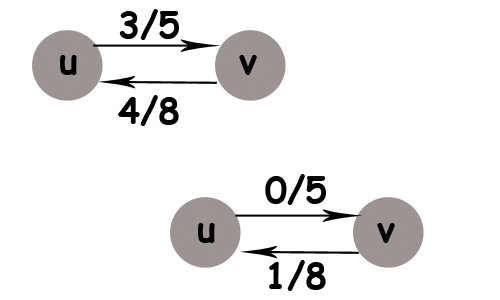
\includegraphics[scale=0.5]{fig2702.png}

\subsection*{Exercise 27.1-2 (1st edition)}
\textbf{Verify the three maximum flow properties for the flow f
shown in Figure 27.1(b)}

Capacity constraint: For all $u, v \epsilon V$, we require $f(u,v)
\leq c(u,v)$.\\
\noindent
$f(s,v_1) = 11\leq 16 = c(s,v_1)$\\
$f(s,v_2) = 8\leq 13 = c(s,v_2)$\\
$f(v_1,v_2) = 0\leq 10 = c(v_1,v_2)$\\
$f(v_1,v_3) = 12\leq 12 = c(v_1,v_3)$\\
$f(v_2,v_1) = 1\leq 4 = c(v_2, v_1)$\\
$f(v_2,v_4) = 11\leq 14 = c(v_2,v_4)$\\
$f(v_3,v_2) = 4\leq 9 = c(v_3,v_2)$\\
$f(v_3,t) = 15\leq 20 = c(v_3,t)$\\
$f(v_4,v_3) = 7\leq 7 = c(v_4,v_3)$\\
$f(v_4,t) = 4\leq 4 = c(v_4,t)$\\

Skew symmetry: For all $u,v\epsilon V$, we require $f(u, v) = - f
(v,u)$.\\
Using $v$\noindent as an iterator over all connected vertices, we
have:
\\

\noindent
%$f(s,v) = 11 + 8 = -(-11-8) = f(v,s)$\\
$f(v_1,v) = 12 = -(-11-1) = f(v,v_1)$\\
$f(v_2,v) = 1 + 11 = -(-8-4) = f(v,v_2)$\\
$f(v_3,v) = 4 + 15 = -(-12-7) = f(v,v_3)$\\
$f(v_4,v) = 7 + 4 = -(-11) = f(v,v_4)$\\
%$f(t,v) = 15 + 4 = -(-4-15) = f(v,t)$\\

Flow conservation: For all $u, v \epsilon V - {s, t}$, we require
$\sum_{u \epsilon V}f(u,v) = 0$.\\

\noindent
$f(v_1,v) + f(v,v_1) = 12 - 1$\\
$f(v_2,v) + f(v,v_2) = 1 + 11 - 4$\\
$f(v_3,v) + f(v,v_3) = 4 - 12 - 7$\\
$f(v_4,v) + f(v,v_4) = 7 - 11$\\

\noindent
$12-1+1+11-4+4-12-7+7-11$\\\\
$12-12-1+1+11-11-4+4-7+7 = 0$\\

\subsection*{Exercise 26.1-5}

\textbf{For the flow network $G = (V, E)$ and flow f shown in Figure
26.1(b), find a pair of subsets $X, Y \subseteq V$ for which $f(X,
Y) = - f(V - X, Y)$. Then, find a pair of subsets $X, Y \subseteq V$
for which $f (X, Y) = - f(V - X, Y)$.}

The trivial case is not excluded. So we have $X = V/{s,t}, Y = V -
{s,t}$, (the set of intermediate vertices). Since $X = Y, f(X,Y) =
0$ because of flow conservation (property 3 from the second page).
We also have $- f(V - X, Y) = 11 + 8 - 15 - 4 = 0 = f(X,Y)$.

Now, for the case where $f(X,Y) \neq - f(V - X, Y)$. The simplest
obvious cut is to remove either the source or sink. So let $X = {t},
Y = V / {t}$. Then $f(X,Y) = -15 - 4 = - 19 \neq 0 = -f(V-X, Y)$
since $V-X = V/{t} = Y$, and is zero by property 3.

\subsection*{Exercise 26.2-1}
\textbf{In Figure 26.1(b), what is the flow across the cut (${s,
v_2, v_4}, {v_1, v_3, t}$)? What is the capacity of this cut?}
The flow is: $11+1-4+7+4 = 19$\\
The capacity is: $16+4+7+4 = 31$ (capacity from former to latter) or $10 + 9 = 19$ (capacity from latter to former)\\
\newpage
\subsection*{Exercises 26.2-2}
\textbf{Show the execution of the Edmunds Karp algorithm on the flow
network of Figure 26.1(a).} I did not show the residual network
because that is simple to see at each step, by reversing the edge
directions. The residual numbers
are given in gray.\\
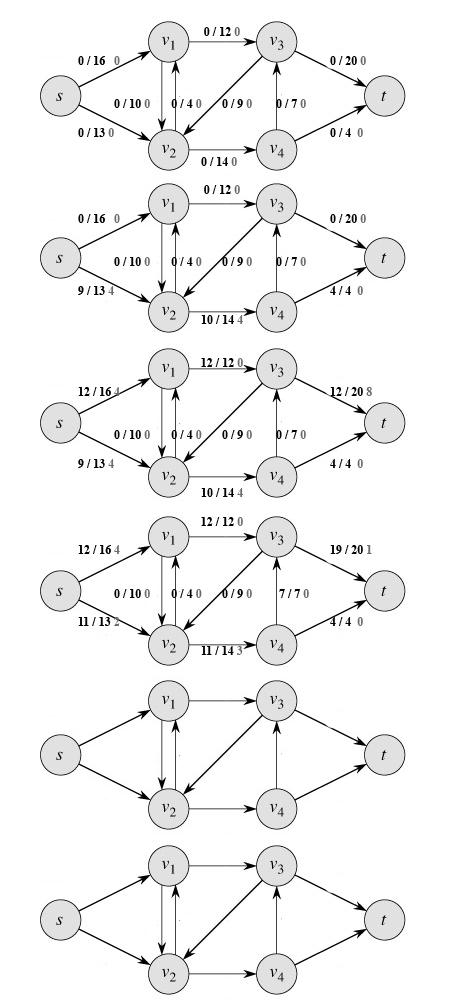
\includegraphics[scale=0.6]{karp2601.png}

\subsection*{Exercises 26.2-3}
\textbf{In the example of Figure 26.5, what is the minimum cut
corresponding to the maximum flow shown? Of the augmenting paths
appearing in the example, which two cancel flow?}

Note that this corresponds to the result obtained in the previous
exercise, since Edmund Karp is an instance of the general Ford
Fulkerson method. The minimum cut which corresponds to the maximum
flow is $( V/{t}, {t} )$ and the flow is $19 + 4 = 23.$ I did not
graphically show the augmenting paths, but those that cancel flow
are $(s,v_1), and (v_3,t)$.

\end{document}
